\documentclass[aspectratio=169,10pt]{beamer}

\mode<presentation>{
  \usetheme[width=0.68in]{Hannover}
  \setbeamercovered{invisible}
}
\usepackage[english]{babel}
\usepackage[utf8]{inputenc}
\usepackage[T1]{fontenc}
\usepackage{times}
\usepackage{booktabs}
\usepackage{array}
\usepackage{listings}
\usepackage{lstlinebgrd}
\usepackage{graphicx}
\usepackage{grffile}
\usepackage{tikz}
\usetikzlibrary{arrows.meta,calc,fit,positioning}

\definecolor{macgold}{RGB}{255,192,0}
\definecolor{templateforest}{RGB}{28,92,62}
\definecolor{templatecalm}{RGB}{218,233,223}
\definecolor{drasilblue}{RGB}{44,103,176}
\definecolor{drasilgreen}{RGB}{27,158,119}
\definecolor{drasilorange}{RGB}{217,95,2}
\definecolor{drasilred}{RGB}{190,35,45}
\definecolor{softgray}{RGB}{245,245,245}
\definecolor{midgray}{RGB}{90,90,90}

\setbeamercolor{structure}{fg=templateforest}
\setbeamercolor{sidebar}{bg=templatecalm}
\setbeamercolor{palette sidebar primary}{fg=templateforest!45!black,bg=templatecalm}
\setbeamercolor{palette sidebar secondary}{fg=templateforest!55!black,bg=templatecalm}
\setbeamercolor{palette sidebar tertiary}{fg=templateforest!65!black,bg=templatecalm}
\setbeamercolor{palette sidebar quaternary}{fg=templateforest!75!black,bg=templatecalm}
\setbeamercolor{section in sidebar}{fg=white,bg=templateforest}
\setbeamercolor{section in sidebar shaded}{fg=templateforest!70!black,bg=templatecalm}
\setbeamercolor{frametitle}{fg=white,bg=templateforest}
\setbeamercolor{block title}{fg=white,bg=templateforest}
\setbeamercolor{block body}{fg=black,bg=softgray}
\setbeamercolor{block title alerted}{fg=white,bg=templateforest}
\setbeamercolor{block body alerted}{fg=black,bg=templatecalm!45!white}
\setbeamercolor{alerted text}{fg=drasilred}
\setbeamertemplate{navigation symbols}{}
\setbeamertemplate{items}[circle]
\setbeamertemplate{frametitle}[default][center]
\makeatletter
\addtobeamertemplate{sidebar left}{}{% 
  \ifnum\value{framenumber}>1\relax
    \begin{beamercolorbox}[wd=\beamer@sidebarwidth,center]{author in sidebar}
      \usebeamerfont{author in sidebar}\tiny
      Daniel M.\\Szymczak
    \end{beamercolorbox}
    \vskip0.8em
  \fi
}
\makeatother

\lstdefinestyle{drasil}{
  backgroundcolor=\color{softgray},
  basicstyle=\ttfamily\scriptsize,
  commentstyle=\color{midgray},
  keywordstyle=\color{drasilblue}\bfseries,
  stringstyle=\color{drasilorange},
  numbers=left,
  numberstyle=\tiny\color{midgray},
  numbersep=5pt,
  frame=single,
  rulecolor=\color{midgray!40},
  breaklines=true,
  columns=fullflexible,
  keepspaces=true,
  showstringspaces=false,
  tabsize=2
}
\lstset{style=drasil}
\newcommand{\DataDefsAssignmentHighlight}{%
  \ifnum\value{lstnumber}=72\relax\color{drasilorange!14}\fi}

\pgfdeclareimage[height=0.62cm]{logo}{McMasterLogo-clean.pdf}
\title[\pgfuseimage{logo}]{Succinctly Verbose: The Drasil Framework}
\subtitle{Ph.D. Defence}
\author[Slide \insertframenumber]{Daniel M. Szymczak}
\institute[McMaster University]{
  Department of Computing and Software\\
  Faculty of Engineering, McMaster University\\[0.35em]
  Supervisors: Jacques Carette and Spencer Smith
}
\date{}

\newcommand{\softifact}{\emph{softifact}}
\newcommand{\softifacts}{\emph{softifacts}}
\newcommand{\qhat}{\ensuremath{\hat{q}}}
\newcommand{\claim}[1]{%
  \begin{center}
    \setlength{\fboxsep}{7pt}%
    \colorbox{drasilblue!9}{\parbox{0.88\linewidth}{\centering #1}}%
  \end{center}
}
\newcommand{\ThesisFigureSlide}[4]{%
  \begin{frame}{Figure #1}
    \centering
    \includegraphics[width=0.98\linewidth,height=0.72\textheight,
      keepaspectratio]{supplementary-figures/fig-#1.pdf}
    \vfill
    {\footnotesize\textbf{Figure #1.} #2\par}
  \end{frame}
}
\newcommand{\Roadmap}[1]{%
\begin{frame}{Talk roadmap}
\begin{center}
\begin{tikzpicture}[node distance=0.34cm,>=Latex,
  roadstep/.style={rounded corners=2pt,minimum width=2.25cm,minimum height=1.18cm,
               align=center,text width=2.05cm}]
  \node[roadstep,draw=drasilred,fill=drasilred!10] (problem)
        {\textbf{Question}\\one fact, many views};
  \node[roadstep,draw=drasilgreen,fill=drasilgreen!10,right=of problem,font=\small] (drasil)
        {\textbf{Approach}\\[-0.1em]\scriptsize(Drasil)\\chunks + recipes\\+ generation};
  \node[roadstep,draw=drasilblue,fill=drasilblue!10,right=of drasil] (walk)
        {\textbf{Example}\\\qhat{} end to end};
  \node[roadstep,draw=drasilorange,fill=drasilorange!10,right=of walk] (evidence)
        {\textbf{Results}\\six case studies};
  \node[roadstep,draw=templateforest,fill=templatecalm,right=of evidence] (answer)
        {\textbf{Answer}\\bounded conclusion};
  \foreach \a/\b in {problem/drasil,drasil/walk,walk/evidence,evidence/answer}
    \draw[->,thick,gray] (\a) -- (\b);
  \node[fit=(#1),draw=drasilorange,very thick,rounded corners=4pt,inner sep=4pt] {};
\end{tikzpicture}
\end{center}
\vspace{0.25em}
\begin{columns}[T,onlytextwidth]
\column{0.32\textwidth}
\textbf{Lens 1: Consistency}\\
Does one change propagate?
\column{0.32\textwidth}
\textbf{Lens 2: Traceability}\\
Can an output be traced to its source?
\column{0.32\textwidth}
\textbf{Lens 3: Reproducibility}\\
Can the artifact set be regenerated?
\end{columns}
\end{frame}
}

\begin{document}

\begin{frame}
  \titlepage
\end{frame}

\section{Question}

\Roadmap{problem}

\begin{frame}[fragile]{One fact, three copies}
\begin{columns}[T,onlytextwidth]
\column{0.31\textwidth}
\begin{block}{Natural language}
\centering\vspace{0.55em}
$P_b$ is the probability of breakage.
\vspace{0.55em}
\end{block}
\column{0.27\textwidth}
\begin{block}{Equation}
\centering\vspace{0.55em}
\Large $P_b = 1-e^{-B}$
\vspace{0.55em}
\end{block}
\column{0.38\textwidth}
\begin{block}{Python}
\begin{lstlisting}[numbers=none,basicstyle=\ttfamily\scriptsize]
def func_P_b(B):
    return 1.0 - math.exp(-B)
\end{lstlisting}
\end{block}
\end{columns}

\vspace{0.65em}
\begin{center}
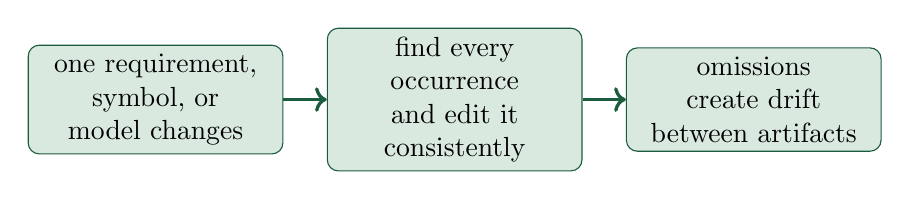
\begin{tikzpicture}[node distance=0.55cm]
\node[draw=templateforest,fill=templatecalm,rounded corners,align=center,text width=3.0cm] (change)
  {one requirement, symbol, or model changes};
\node[draw=templateforest,fill=templatecalm,rounded corners,align=center,text width=3.0cm,right=of change] (work)
  {find every occurrence\\and edit it consistently};
\node[draw=templateforest,fill=templatecalm,rounded corners,align=center,text width=3.0cm,right=of work] (risk)
  {omissions create drift\\between artifacts};
\draw[->,very thick,templateforest] (change) -- (work);
\draw[->,very thick,templateforest] (work) -- (risk);
\end{tikzpicture}
\end{center}
\end{frame}

\begin{frame}{Question and scope}
\begin{block}{Motivating question}
\large
How can we systematically reduce unnecessary redundancy and improve consistency
across \softifacts{}, especially where correctness and traceability are critical?
\end{block}

\vspace{0.35em}
\begin{columns}[T,onlytextwidth]
\column{0.49\textwidth}
\textbf{In scope}
\begin{itemize}
  \item well-understood scientific software
  \item input $\rightarrow$ compute $\rightarrow$ output systems
  \item requirements, source code, and build instructions
  \item long-lived systems with shared knowledge
\end{itemize}
\column{0.49\textwidth}
\textbf{Not claimed}
\begin{itemize}
  \item generation of every possible artifact
  \item elimination of repeated presentation
  \item controlled proof of human productivity or defect reduction
  \item present coverage of highly dynamic or stateful systems
\end{itemize}
\end{columns}
\end{frame}

\section{Approach}

\Roadmap{drasil}

\begin{frame}{Ideas that shaped Drasil}
\begin{center}
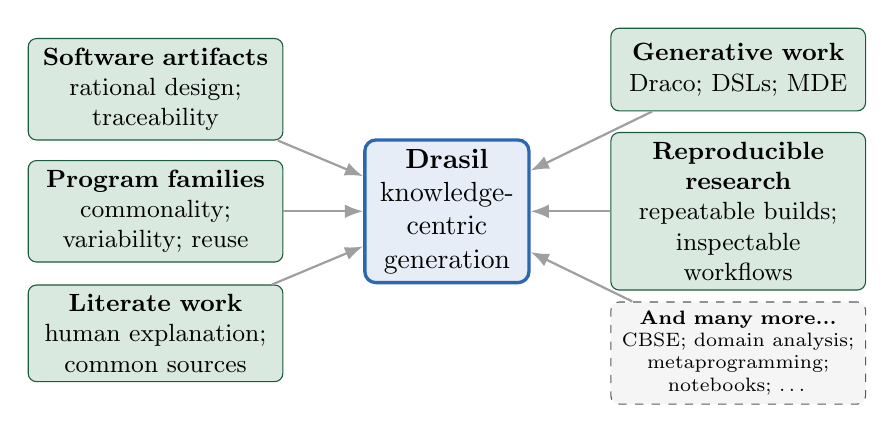
\begin{tikzpicture}[>=Latex,
  influence/.style={draw=templateforest,fill=templatecalm,rounded corners=3pt,
    align=center,text width=3.0cm,minimum height=1.05cm,font=\small},
  core/.style={draw=drasilblue,fill=drasilblue!12,very thick,rounded corners=4pt,
    align=center,text width=1.85cm,minimum height=1.15cm}]
\node[core] (drasil) at (0,0) {\textbf{Drasil}\\knowledge-centric\\generation};
\node[influence] (artifacts) at (-3.7,1.55)
  {\textbf{Software artifacts}\\rational design; traceability};
\node[influence] (families) at (-3.7,0)
  {\textbf{Program families}\\commonality; variability; reuse};
\node[influence] (literate) at (-3.7,-1.55)
  {\textbf{Literate work}\\human explanation;\\common sources};
\node[influence] (generative) at (3.7,1.8)
  {\textbf{Generative work}\\Draco; DSLs; MDE};
\node[influence] (repro) at (3.7,0)
  {\textbf{Reproducible research}\\repeatable builds;\\inspectable workflows};
\node[influence,draw=midgray,fill=softgray,dashed,font=\scriptsize] (more) at (3.7,-1.8)
  {\textbf{And many more...}\\CBSE; domain analysis;\\metaprogramming; notebooks; \ldots};
\foreach \n in {artifacts,families,literate,generative,repro,more}
  \draw[->,thick,gray!75] (\n) -- (drasil);
\end{tikzpicture}
\end{center}
\vspace{-0.15em}
\claim{Drasil combines complementary lessons from these traditions; no single one is its theoretical foundation.}
\end{frame}

\begin{frame}{Drasil at a glance}
\begin{center}
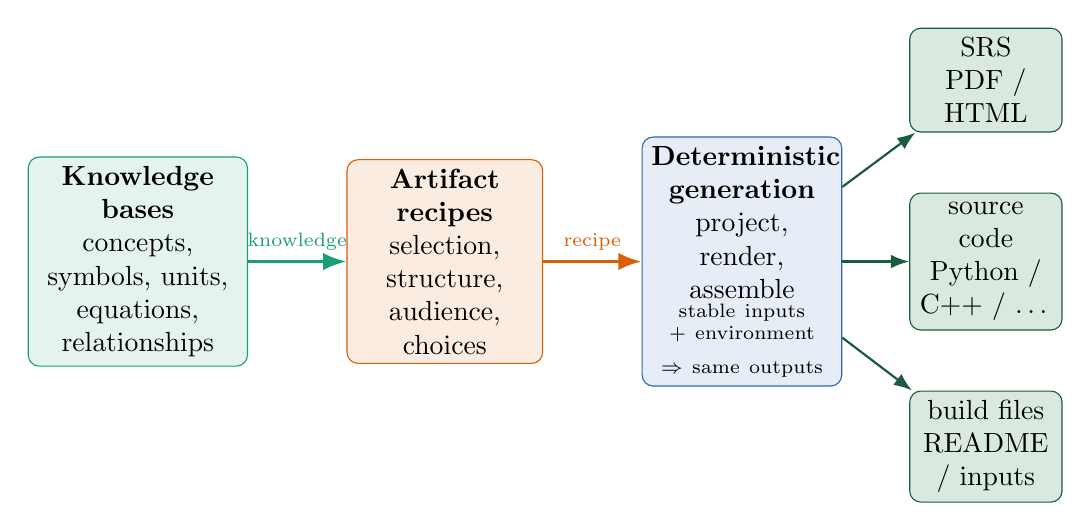
\begin{tikzpicture}[>=Latex,node distance=0.72cm and 1.25cm]
\node[draw=drasilgreen,fill=drasilgreen!12,rounded corners,minimum height=2.05cm,
      text width=2.55cm,align=center] (kb)
      {\textbf{Knowledge bases}\\concepts, symbols, units, equations, relationships};
\node[draw=drasilorange,fill=drasilorange!12,rounded corners,minimum height=2.05cm,
      text width=2.25cm,align=center,right=of kb] (recipes)
      {\textbf{Artifact recipes}\\selection, structure, audience, choices};
\node[draw=drasilblue,fill=drasilblue!12,rounded corners,minimum height=2.05cm,
      text width=2.3cm,align=center,right=of recipes] (gen)
      {\textbf{Deterministic generation}\\project, render, assemble\\[-0.1em]
       \scriptsize stable inputs + environment\\$\Rightarrow$ same outputs};
\node[draw=templateforest,fill=templatecalm,rounded corners,text width=1.7cm,
      align=center,above right=0.05cm and 0.85cm of gen] (srs) {SRS\\PDF / HTML};
\node[draw=templateforest,fill=templatecalm,rounded corners,text width=1.7cm,
      align=center,right=0.85cm of gen] (code) {source code\\Python / C++ / \ldots};
\node[draw=templateforest,fill=templatecalm,rounded corners,text width=1.7cm,
      align=center,below right=0.05cm and 0.85cm of gen] (aux) {build files\\README / inputs};
\draw[->,very thick,drasilgreen] (kb) -- node[above,font=\scriptsize]{knowledge} (recipes);
\draw[->,very thick,drasilorange] (recipes) -- node[above,font=\scriptsize]{recipe} (gen);
\draw[->,thick,templateforest] (gen) -- (srs);
\draw[->,thick,templateforest] (gen) -- (code);
\draw[->,thick,templateforest] (gen) -- (aux);
\end{tikzpicture}
\end{center}
{\small
\claim{The authoritative sources are the captured knowledge and recipes---not each rendered occurrence.}}
\end{frame}

\begin{frame}{Four key terms}
\begin{columns}[T,onlytextwidth]
\column{0.48\textwidth}
\begin{block}{Chunk}
A named, reusable unit of knowledge: for example, a concept, quantity,
definition, unit, equation, or relation.
\end{block}
\begin{block}{Recipe}
Specifies which chunks an artifact needs and how they are organized for a
particular purpose and audience.
\end{block}
\column{0.48\textwidth}
\begin{block}{Projection}
Selects the relevant view of captured knowledge: a symbol table entry, a full
definition, or an executable expression.
\end{block}
\begin{block}{\softifact}
Any software-development artifact that conveys knowledge, including
requirements, designs, code, tests, manuals, and build instructions.
\end{block}
\end{columns}
\end{frame}

\section{Example}

\Roadmap{walk}

\begin{frame}{Running example: GlassBR \& \qhat{}}
\begin{columns}[c,onlytextwidth]
\column{0.46\textwidth}
\begin{block}{GlassBR}
Predict whether a glass slab can withstand a specified blast load.
\end{block}
\begin{itemize}
  \item \qhat{} is a dimensionless quantity used in later GlassBR calculations.
  \item It combines applied load, plate dimensions, material properties,
        thickness, and glass type.
  \item It appears differently in reference material, data definitions, and code.
\end{itemize}
\column{0.50\textwidth}
\begin{center}
\Large
\[
\color{drasilblue}{\boxed{\qhat}}
= \frac{q(ab)^2}{E h^4\,\mathit{GTF}}
\]
\normalsize
\end{center}
\vspace{0.8em}
\begin{center}
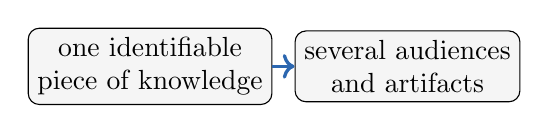
\begin{tikzpicture}[node distance=0.28cm]
\node[draw,rounded corners,fill=softgray,align=center] (one)
  {one identifiable\\piece of knowledge};
\node[draw,rounded corners,fill=softgray,align=center,right=of one] (many)
  {several audiences\\and artifacts};
\draw[->,very thick,drasilblue] (one) -- (many);
\end{tikzpicture}
\end{center}
\end{columns}
\end{frame}

\begin{frame}[fragile]{1. Capture \qhat{} once}
\begin{columns}[T,onlytextwidth]
\column{0.67\textwidth}
\lstinputlisting[language=Haskell,firstline=132,lastline=141,firstnumber=132,
  emph={dimLL},emphstyle={\color{drasilgreen!70!black}\bfseries}]{../Draft/code/DataDefs.hs}
\column{0.30\textwidth}
\textbf{The chunk connects}
\begin{itemize}
  \item canonical identity
  \item defining expression
  \item referenced symbol and description
  \item sources
  \item notes and relations
\end{itemize}
\vspace{0.4em}
\colorbox{drasilblue!12}{\parbox{0.88\linewidth}{\centering
\textbf{Authority:} \texttt{dimLL}\\[-0.1em]}}
\end{columns}
\end{frame}

\begin{frame}[fragile]{2. Select \qhat{} with recipes}
\begin{columns}[T,onlytextwidth]
\column{0.48\textwidth}
\textbf{System information}
\lstinputlisting[language=Haskell,firstline=63,lastline=78,firstnumber=63,
  basicstyle=\ttfamily\tiny,
  emph={_datadefs,GB,dataDefs},emphstyle={\color{drasilorange!80!black}\bfseries},
  linebackgroundcolor=\DataDefsAssignmentHighlight]{../Draft/code/Body.hs}
\column{0.48\textwidth}
\textbf{GlassBR data definitions}
\lstinputlisting[language=Haskell,firstline=34,lastline=37,firstnumber=34,
  emph={dimLL},emphstyle={\color{drasilgreen!70!black}\bfseries}]{../Draft/code/DataDefs.hs}
\vspace{0.7em}
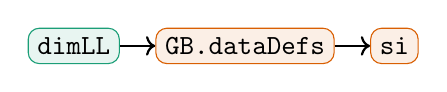
\begin{tikzpicture}[node distance=0.45cm]
\node[draw=drasilgreen,fill=drasilgreen!10,rounded corners] (chunk) {\texttt{dimLL}};
\node[draw=drasilorange,fill=drasilorange!10,rounded corners,right=of chunk] (list) {\texttt{GB.dataDefs}};
\node[draw=drasilorange,fill=drasilorange!10,rounded corners,right=of list] (si) {\texttt{si}};
\draw[->,thick] (chunk)--(list);
\draw[->,thick] (list)--(si);
\end{tikzpicture}
\end{columns}
\end{frame}

\begin{frame}{3. Project for each audience}
\begin{center}
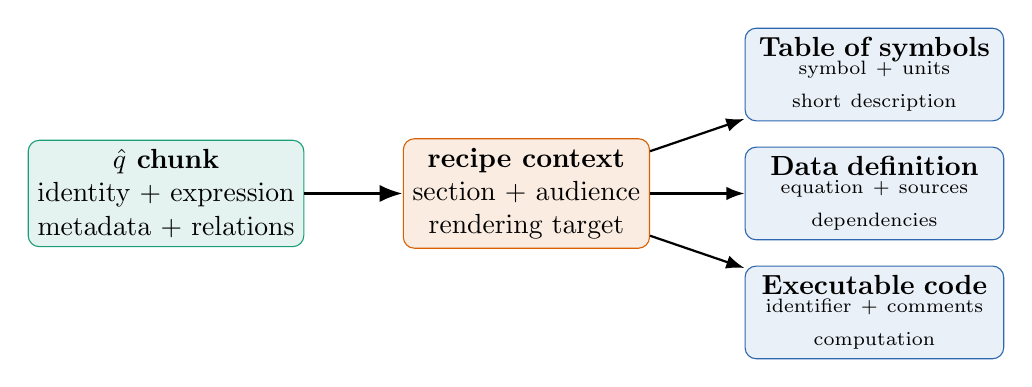
\begin{tikzpicture}[>=Latex,node distance=0.6cm and 1.25cm]
\node[draw=drasilgreen,fill=drasilgreen!12,rounded corners,minimum width=2.3cm,
      minimum height=1.2cm,align=center] (chunk) {\textbf{\qhat{} chunk}\\identity + expression\\metadata + relations};
\node[draw=drasilorange,fill=drasilorange!12,rounded corners,right=of chunk,
      minimum height=1.2cm,align=center] (recipe) {\textbf{recipe context}\\section + audience\\rendering target};
\node[draw=drasilblue,fill=drasilblue!10,rounded corners,right=1.2cm of recipe,
      text width=3.05cm,minimum height=0.85cm,align=center] (dd)
      {\textbf{Data definition}\\[-0.15em]\scriptsize equation + sources\\dependencies};
\node[draw=drasilblue,fill=drasilblue!10,rounded corners,above=0.32cm of dd,
      text width=3.05cm,minimum height=0.85cm,align=center] (symbols)
      {\textbf{Table of symbols}\\[-0.15em]\scriptsize symbol + units\\short description};
\node[draw=drasilblue,fill=drasilblue!10,rounded corners,below=0.32cm of dd,
      text width=3.05cm,minimum height=0.85cm,align=center] (code)
      {\textbf{Executable code}\\[-0.15em]\scriptsize identifier + comments\\computation};
\draw[->,very thick] (chunk)--(recipe);
\draw[->,thick] (recipe)--(symbols);
\draw[->,thick] (recipe)--(dd);
\draw[->,thick] (recipe)--(code);
\end{tikzpicture}
\end{center}
\claim{Different representations are expected; independent meanings are not.}
\end{frame}

\begin{frame}{4. Generate the SRS}
\centering
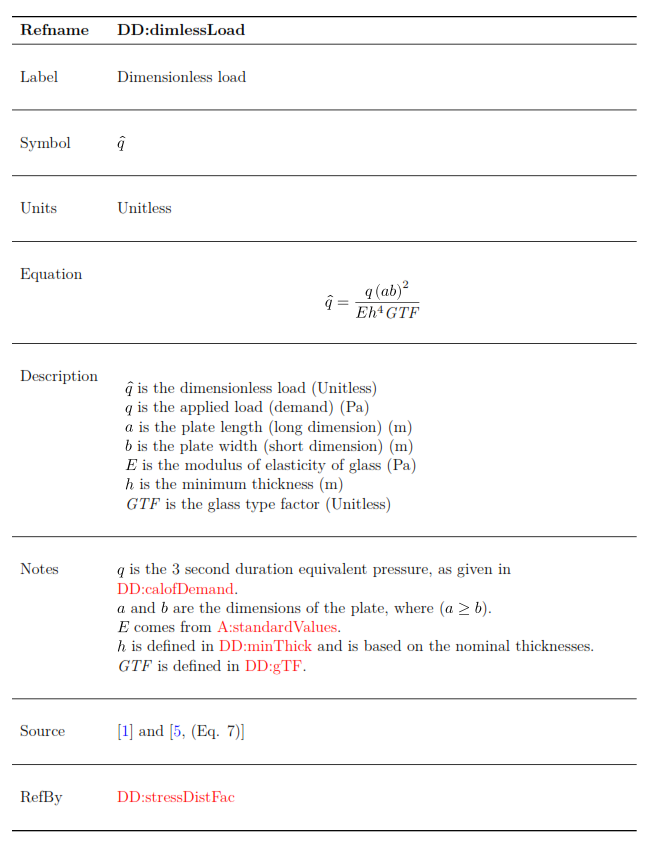
\includegraphics[height=0.82\textheight]{../Draft/figures/dimensionless_load.png}
\end{frame}

\begin{frame}[fragile]{5. Generate Python}
\begin{columns}[c,onlytextwidth]
\column{0.48\textwidth}
\begin{center}
\Large
\[
\color{drasilblue}{\qhat}
= \frac{q(ab)^2}{E h^4\,\mathit{GTF}}
\]
\normalsize
captured mathematical relation
\end{center}
\column{0.49\textwidth}
\lstinputlisting[language=Python,firstline=34,lastline=40,firstnumber=34]{../Draft/code/GenCalculations.py}
\end{columns}

\vspace{0.5em}
\begin{center}
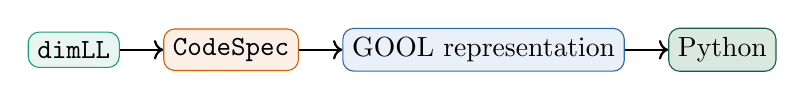
\begin{tikzpicture}[node distance=0.55cm]
\node[draw=drasilgreen,fill=drasilgreen!10,rounded corners] (source) {\texttt{dimLL}};
\node[draw=drasilorange,fill=drasilorange!10,rounded corners,right=of source] (spec) {\texttt{CodeSpec}};
\node[draw=drasilblue,fill=drasilblue!10,rounded corners,right=of spec] (gool) {GOOL representation};
\node[draw=templateforest,fill=templatecalm,rounded corners,right=of gool] (py) {Python};
\foreach \a/\b in {source/spec,spec/gool,gool/py}\draw[->,thick](\a)--(\b);
\end{tikzpicture}
\end{center}
\end{frame}

\begin{frame}{Localizing maintenance}
\begin{center}
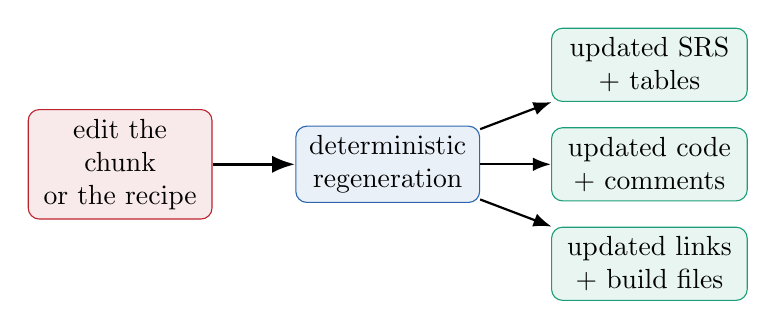
\begin{tikzpicture}[>=Latex,node distance=0.7cm and 1.05cm]
\node[draw=drasilred,fill=drasilred!10,rounded corners,align=center,text width=2.1cm] (edit)
  {edit the chunk\\or the recipe};
\node[draw=drasilblue,fill=drasilblue!10,rounded corners,align=center,right=of edit,text width=2.1cm] (regen)
  {deterministic\\regeneration};
\node[draw=drasilgreen,fill=drasilgreen!10,rounded corners,align=center,
      right=0.9cm of regen,text width=2.25cm,minimum height=0.78cm] (code)
  {updated code + comments};
\node[draw=drasilgreen,fill=drasilgreen!10,rounded corners,align=center,
      above=0.32cm of code,text width=2.25cm,minimum height=0.78cm] (doc)
  {updated SRS + tables};
\node[draw=drasilgreen,fill=drasilgreen!10,rounded corners,align=center,
      below=0.32cm of code,text width=2.25cm,minimum height=0.78cm] (trace)
  {updated links + build files};
\draw[->,very thick] (edit)--(regen);
\draw[->,thick] (regen)--(doc);
\draw[->,thick] (regen)--(code);
\draw[->,thick] (regen)--(trace);
\end{tikzpicture}
\end{center}

\begin{block}{Consequential choice}
Knowledge capture is separated from artifact-specific presentation. A change
is made at the authoritative source and then propagated by regeneration.
\end{block}
\end{frame}

\section{Results}

\Roadmap{evidence}

\begin{frame}{Case study reimplementations}
\small
\begin{center}
\begin{tabular}{lrrrr}
\toprule
\textbf{Case study} & \textbf{SRS pages} & \textbf{Example Haskell} & \textbf{SRS TeX} & \textbf{Generated code}\\
\midrule
GlassBR      & 44 & 1,651 & 1,778 & 7,625\\
SWHS         & 50 & 2,273 & 1,949 & --\\
NoPCM        & 32 &   674 & 1,209 & 1,760\\
SSP          & 84 & 3,036 & 2,993 & --\\
Projectile   & 31 & 1,377 & 1,244 & 4,768\\
GamePhysics  & 46 & 2,029 & 1,841 & --\\
\midrule
\textbf{Total} & \textbf{287} & \textbf{11,040} & \textbf{11,014} & \textbf{14,153}\\
\bottomrule
\end{tabular}
\end{center}

\begin{itemize}
  \item All six use shared Drasil infrastructure (about 44,269 Haskell LOC in the thesis snapshot).
  \item Reimplementation required recovering, resolving, and structuring concepts,
        assumptions, equations, dependencies, commonalities, and variations.
  \item The counts demonstrate nontrivial generated artifacts; they do not by themselves measure productivity.
\end{itemize}
\end{frame}

\begin{frame}{Case-study findings}
\small
\begin{columns}[T,onlytextwidth]
\column{0.32\textwidth}
\begin{block}{Consistency}
\begin{minipage}[t][2.35cm][t]{\linewidth}
\raggedright
Local knowledge or recipe edits propagated to generated documentation and code,
removing separate synchronization tasks.
\end{minipage}
\end{block}
\column{0.32\textwidth}
\begin{block}{Traceability}
\begin{minipage}[t][2.35cm][t]{\linewidth}
\raggedright
Named chunks, recipes, references, and generated matrices exposed provenance and
made the source of a definition or relation easier to locate.
\end{minipage}
\end{block}
\column{0.32\textwidth}
\begin{block}{Reproducibility}
\begin{minipage}[t][2.35cm][t]{\linewidth}
\raggedright
From the same knowledge base and recipes, regression checks confirmed
byte-for-byte equivalent stable outputs in environment-consistent builds.
\end{minipage}
\end{block}
\end{columns}

\vspace{0.65em}
\claim{These are observational results from reimplementation, not controlled measurements of productivity, maintenance cost, or defect reduction.}
\end{frame}

\begin{frame}{Making problems visible}
\begin{columns}[T,onlytextwidth]
\column{0.48\textwidth}
\begin{block}{Issue \#348 (SSP)}
Encoding related shear-stress quantities exposed conflicting identifiers,
missing definitions, and an undocumented 1 m ``into the page'' assumption.
\end{block}
\textbf{Observed effect:} correcting the underlying chunks removed the
inconsistencies from generated artifacts after regeneration.
\column{0.48\textwidth}
\begin{block}{Issue \#363 (GlassBR)}
Traceability localized an implicit unit conversion. The conversion was made
explicit in the source chunk rather than left hidden in a rendered equation.
\end{block}
\textbf{Observed effect:} the corrected expression propagated to the SRS and
generated computations.
\end{columns}
\vspace{0.55em}
\claim{Centralization does not prevent a bad source; it makes the source reviewable and a correction single-point.}
\end{frame}

\begin{frame}{Software-family reuse}
\small
\begin{center}
\begin{tabular}{lcc}
\toprule
\textbf{Captured element} & \textbf{SWHS} & \textbf{NoPCM}\\
\midrule
Tank and water properties & shared & shared\\
Sensible heat             & included & included\\
Energy-balance structure  & included & included\\
PCM properties and inputs & included & excluded\\
Latent heat               & included & excluded\\
PCM assumptions           & included & excluded\\
\midrule
Artifact recipe           & include PCM chunks & omit PCM chunks\\
\bottomrule
\end{tabular}
\end{center}
\vspace{0.35em}
\begin{itemize}
  \item Shared knowledge and recipe structure were retained.
  \item The variant is expressed by selecting the relevant chunks, not by rewriting the common specification.
  \item This is controlled reuse, not a claim that every family variation is automatically inferred.
\end{itemize}
\end{frame}

\begin{frame}{Costs and limits}
\small
\begin{columns}[T,onlytextwidth]
\column{0.45\textwidth}
\textbf{Up-front cost}
\begin{itemize}
  \item explicit modelling and domain familiarity
  \item learning chunk combinators and recipe patterns
  \item finding existing chunks of the appropriate type
  \item up to two weeks of mentoring in observed onboarding
\end{itemize}
\hfill
\column{0.45\textwidth}
\textbf{Evidence boundary}
\begin{itemize}
  \item results are largely qualitative and anecdotal
  \item current fit: structured, well-understood scientific domains
  \item knowledge discovery and organization become harder at scale
  \item dynamic, event-driven, and stateful systems remain open
\end{itemize}
\end{columns}
\end{frame}

\begin{frame}{Future work}
\small
\begin{tabular}{>{\raggedright\arraybackslash}p{0.36\linewidth} >{\raggedright\arraybackslash}p{0.57\linewidth}}
\toprule
\textbf{Observed limitation} & \textbf{Next direction}\\
\midrule
Modelling and onboarding cost & guided authoring, IDE support, knowledge search and navigation\\[0.35em]
Many relations must be explicit & automatic dependency discovery from captured knowledge\\[0.35em]
Limited deep sanity checks & a typed expression language for stronger model, unit, and dimension validation\\[0.35em]
Qualitative evidence & controlled studies of onboarding, maintenance effort, and defect detection\\[0.35em]
Narrow artifact/domain coverage & more output formats and artifact types; richer knowledge for dynamic systems\\
\bottomrule
\end{tabular}

\vspace{0.45em}
\begin{alertblock}{Current versus proposed guarantee}
Current work provides structured expressions, explicit units, and observed
sanity-checking benefits. Stronger type- and dimension-driven guarantees are
future work.
\end{alertblock}
\end{frame}

\section{Answer}

\Roadmap{answer}

\begin{frame}{Answer}
\begin{quote}
\small\itshape\raggedright
\hyphenpenalty=10000
``How can we systematically reduce unnecessary redundancy and improve consistency
across \softifacts{}, especially where correctness and traceability are critical?''
\end{quote}

\begin{beamercolorbox}[sep=0.7em,wd=\textwidth]{block body alerted}
\large
\textcolor{drasilgreen}{\textbf{Capture shared knowledge once}},
\textcolor{drasilblue}{\textbf{use recipes to define the required views}},
and \textcolor{drasilorange}{\textbf{deterministically generate those views}}
with explicit provenance.
\end{beamercolorbox}

\vspace{0.15em}
{\centering
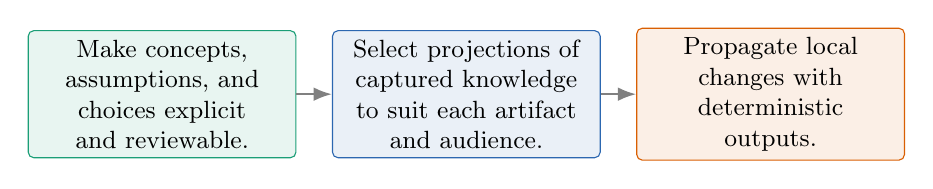
\begin{tikzpicture}[>=Latex,node distance=0.45cm,
  answerstep/.style={rounded corners=2pt,minimum width=3.4cm,
    minimum height=1.45cm,align=center,text width=3.1cm,font=\small,
    execute at begin node={\hyphenpenalty=10000\relax}}]
\node[answerstep,draw=drasilgreen,fill=drasilgreen!10] (capture)
  {Make concepts, assumptions, and choices explicit and reviewable.};
\node[answerstep,draw=drasilblue,fill=drasilblue!10,right=of capture] (project)
  {Select projections of captured knowledge to suit each artifact and audience.};
\node[answerstep,draw=drasilorange,fill=drasilorange!10,right=of project] (generate)
  {Propagate local changes with deterministic outputs.};
\draw[->,thick,gray] (capture) -- (project);
\draw[->,thick,gray] (project) -- (generate);
\end{tikzpicture}
\par}

\vspace{0.35em}
\claim{Drasil moves authority from repeated occurrences to captured knowledge and recipes. It trades up-front modelling for less independent maintenance downstream.}
\end{frame}

\begin{frame}{Contributions}
\begin{columns}[T,onlytextwidth]
\column{0.48\textwidth}
\begin{block}{1. Analyze and operationalize}
Identified recurring knowledge, structure, and variation across scientific
software artifacts and turned that analysis into knowledge-centric generation.
\end{block}
\begin{block}{2. Design and implement}
Developed Drasil's chunk, recipe, projection, rendering, and assembly
architecture for multi-format artifacts.
\end{block}
\column{0.48\textwidth}
\begin{block}{3. Establish observational evidence}
Reimplementations demonstrate consistency by construction, explicit provenance,
deterministic regeneration, and increased visibility of tacit knowledge.
\end{block}
\begin{block}{4. Demonstrate controlled reuse}
Separated knowledge from presentation and produced software-family variants by
selecting and extending shared knowledge rather than duplicating it.
\end{block}
\end{columns}
\end{frame}

\appendix
\section{Supplementary}

\begin{frame}
\vfill
\begin{center}
{\usebeamercolor[fg]{structure}\Huge\bfseries Supplementary Material\par}
\vspace{0.75em}

\begin{tikzpicture}
  \draw[line width=2pt,drasilgreen] (0,0) -- (1.5,0);
  \draw[line width=2pt,drasilblue] (1.7,0) -- (3.2,0);
  \draw[line width=2pt,drasilorange] (3.4,0) -- (4.9,0);
\end{tikzpicture}
\vspace{0.75em}

{\large Additional evidence and discussion\par}
\end{center}
\vfill
\end{frame}

\begin{frame}{Backup: redundancy across GlassBR artifacts}
\centering
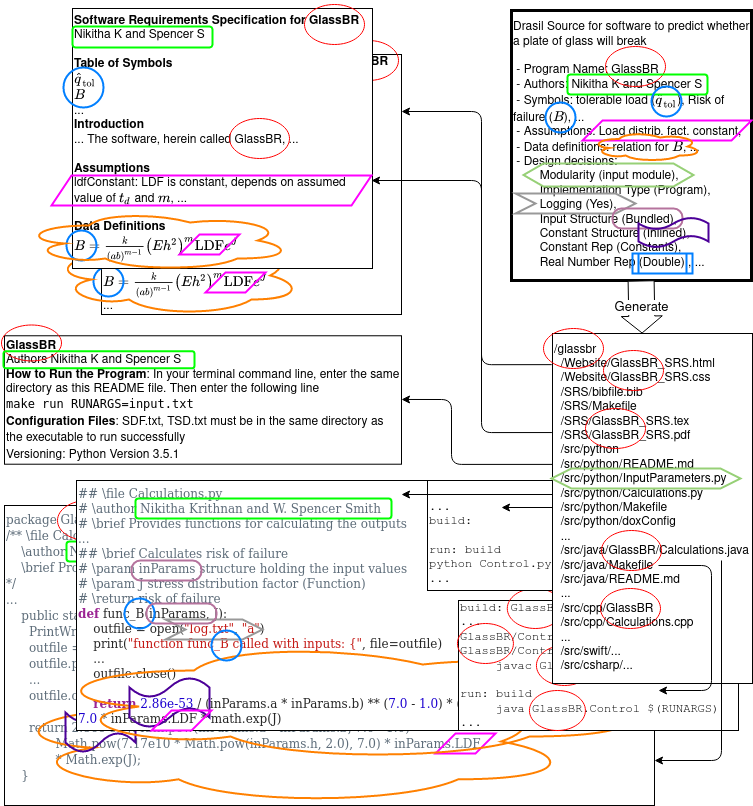
\includegraphics[height=0.82\textheight]{supplementary-figures/CaseStudyRedundancy.png}
\end{frame}

\begin{frame}{Backup: the knowledge footprint of \qhat{}}
\begin{center}
\Large
\color{drasilblue}{$\displaystyle\boxed{\qhat=\frac{q(ab)^2}{E h^4\,\mathit{GTF}}}$}
\end{center}
\vspace{0.25em}
\small
\begin{columns}[T,onlytextwidth]
\column{0.31\textwidth}
\begin{block}{Scientific basis}
\begin{itemize}
  \item plate and blast-load theory
  \item model-selection rationale
  \item ASTM and Campidelli Eq. 7
\end{itemize}
\end{block}
\column{0.31\textwidth}
\begin{block}{Referenced knowledge}
\begin{itemize}
  \item $q,a,b,E,h,\mathit{GTF}$
  \item definitions and symbols
  \item units and constraints
\end{itemize}
\end{block}
\column{0.31\textwidth}
\begin{block}{Relationships}
\begin{itemize}
  \item $q$ is a 3-second equivalent pressure
  \item $a\geq b$
  \item feeds stress-distribution calculations
\end{itemize}
\end{block}
\end{columns}
\vspace{0.4em}
\claim{The chunk is a named connection into this knowledge network, not an isolated formula string.}
\end{frame}

\begin{frame}{Backup: two different generation contracts}
\small
\renewcommand{\arraystretch}{1.22}
\begin{tabular}{>{\raggedright\arraybackslash}p{0.20\linewidth}
                >{\raggedright\arraybackslash}p{0.34\linewidth}
                >{\raggedright\arraybackslash}p{0.36\linewidth}}
\toprule
\textbf{Question} & \textbf{Ordinary prompted generation} & \textbf{Drasil regeneration}\\
\midrule
What drives it? & prompt, supplied context, and model & named knowledge chunks, recipes, and generation choices\\[0.3em]
What happens after a change? & request and review a new response & regenerate every selected projection\\[0.3em]
What repeats? & output may vary across runs or model versions & stable inputs and environment reproduce stable outputs\\[0.3em]
What is connected? & connections depend on supplied context and workflow & definitions, relations, sources, recipes, and outputs remain explicitly linked\\
\bottomrule
\end{tabular}
\vspace{0.45em}
\claim{The distinction is maintained, deterministic projection---not whether a useful artifact can be generated once.}
\end{frame}

\begin{frame}{Backup: influence map in more detail}
\scriptsize
\renewcommand{\arraystretch}{1.18}
\begin{tabular}{>{\raggedright\arraybackslash}p{0.24\linewidth}
                >{\raggedright\arraybackslash}p{0.29\linewidth}
                >{\raggedright\arraybackslash}p{0.37\linewidth}}
\toprule
\textbf{Tradition} & \textbf{Lesson carried forward} & \textbf{Drasil emphasis}\\
\midrule
Artifacts, rational design, traceability & stakeholders need related representations whose relationships survive change & capture shared authority while retaining audience-specific artifacts\\[0.35em]
Program families and commonality analysis & identify commonality and variability explicitly & reuse knowledge and recipes across related systems\\[0.35em]
Literate approaches & organize executable and explanatory material for human understanding & project more than a program and its accompanying narrative\\[0.35em]
Reproducible research & preserve enough code, data, dependencies, and build information to rerun work & combine deterministic generation with explicit domain knowledge\\[0.35em]
Draco, generative programming, DSLs, and MDE & derive concrete software from higher-level domain representations & generate several traceably connected artifact types from fine-grained knowledge\\
\bottomrule
\end{tabular}
\vspace{0.3em}
\begin{center}
\footnotesize Representative anchors include Parnas, Gotel and Finkelstein, Weiss, Kang, Knuth, Neighbors, and Czarnecki.
\end{center}
\end{frame}

\begin{frame}{Backup: contribution boundary}
\small
\begin{columns}[T,onlytextwidth]
\column{0.48\textwidth}
\begin{block}{Principal thesis contributions}
\begin{itemize}
  \item systematic analysis of redundancy and inconsistency
  \item thesis account of the chunk- and recipe-based architecture
  \item substantial framework and representation implementation
  \item case-study reimplementation and evaluation
\end{itemize}
\end{block}
\column{0.48\textwidth}
\begin{block}{Prior and collaborative context}
\begin{itemize}
  \item Drasil is a broader ongoing research project
  \item most original case studies were developed by other teams
  \item GOOL was not developed as part of this thesis
  \item templates, artifacts, guidance, and infrastructure informed the work
\end{itemize}
\end{block}
\end{columns}
\claim{The thesis contribution is the analysis and knowledge-centric realization evaluated here, not sole authorship of every input or subsystem.}
\end{frame}

\begin{frame}{Evidence map}
\small
\renewcommand{\arraystretch}{1.22}
\begin{tabular}{>{\raggedright\arraybackslash}p{0.24\linewidth} >{\raggedright\arraybackslash}p{0.31\linewidth} >{\raggedright\arraybackslash}p{0.34\linewidth}}
\toprule
\textbf{Lens} & \textbf{Slide-level answer} & \textbf{Thesis evidence}\\
\midrule
Consistency & local edits regenerate all selected occurrences & Results: consistency by construction; GlassBR \#363\\[0.4em]
Traceability & outputs retain named sources and generated relationships & Drasil walkthrough; Results: traceability and maintainability\\[0.4em]
Reproducibility & same sources and recipes reproduce stable outputs & Results: deterministic diff-based regression checks\\[0.4em]
Applicability & useful within the studied structured scientific systems & six reimplementations; Discussion and Conclusion limitations\\
\bottomrule
\end{tabular}
\end{frame}

\begin{frame}{Backup: current vs. legacy definition}
\begin{columns}[c,onlytextwidth]
\column{0.45\textwidth}
\centering
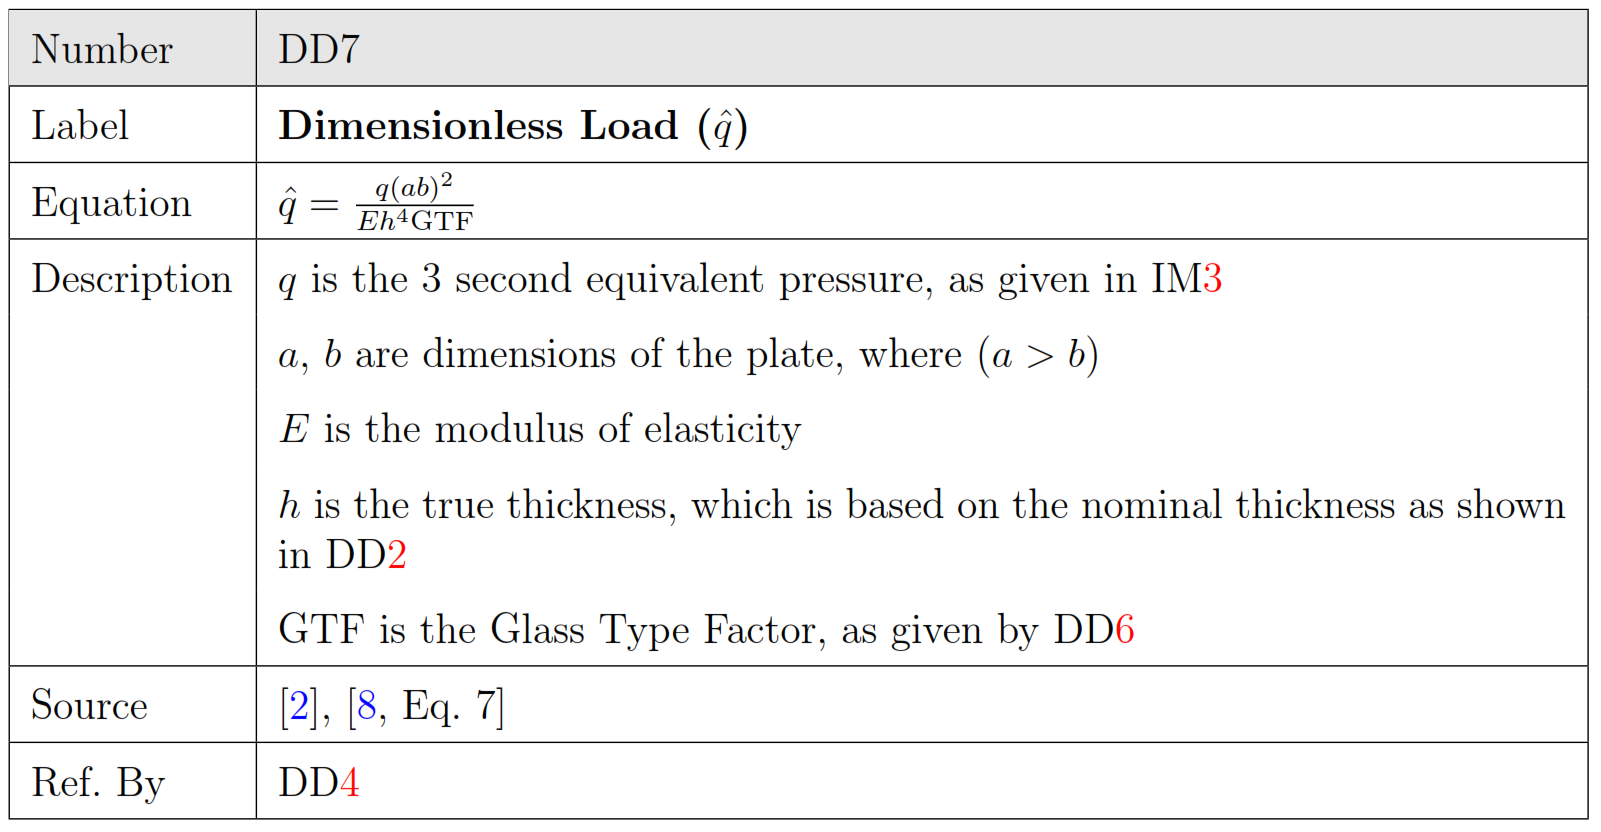
\includegraphics[width=\linewidth]{../Draft/figures/gb_dd_q.png}
\\[-0.2em]\scriptsize Legacy GlassBR data-definition presentation
\column{0.51\textwidth}
\centering
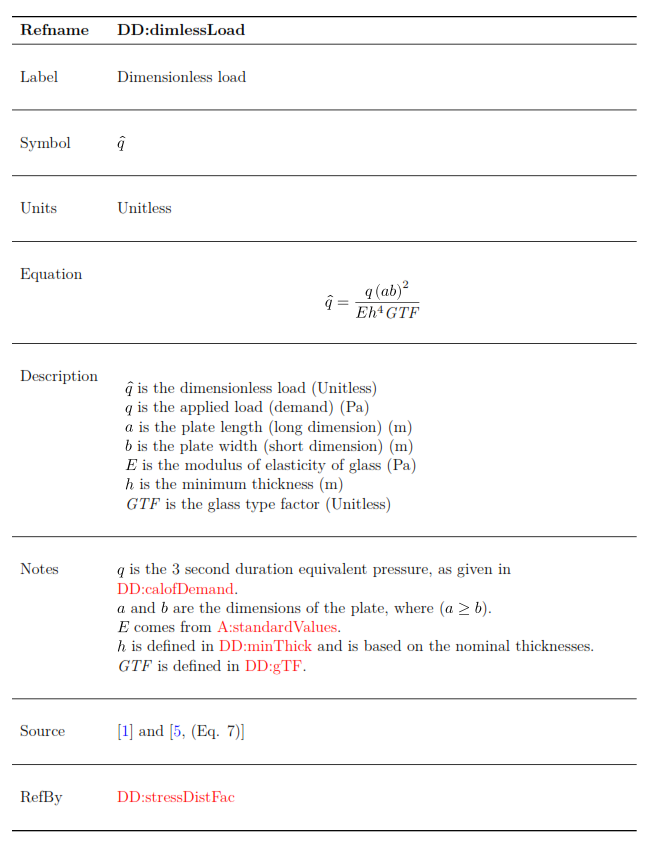
\includegraphics[width=0.82\linewidth]{../Draft/figures/dimensionless_load.png}
\\[-0.2em]\scriptsize Current generated Drasil presentation
\end{columns}
\end{frame}

\ThesisFigureSlide{2.1}{The Waterfall model, used as a historical reference point for common software artifact roles}{28}{85 324 85 122}

\ThesisFigureSlide{3.1}{Table of contents from the expanded Smith et al. template}{51}{95 145 95 115}
\ThesisFigureSlide{3.2}{Table of units section from the GlassBR SRS}{52}{75 300 75 310}
\ThesisFigureSlide{3.3}{Table of symbols (truncated) section from the GlassBR SRS}{53}{75 430 75 95}
\ThesisFigureSlide{3.4}{Abbreviations and acronyms (truncated) section from the GlassBR SRS}{53}{75 115 75 400}
\ThesisFigureSlide{3.5}{Table of contents for the GlassBR Module Guide}{56}{80 150 80 160}
\ThesisFigureSlide{3.6}{Calc module from the GlassBR Module Guide}{57}{75 550 75 120}
\ThesisFigureSlide{3.7}{Python source code directory structure for GlassBR}{58}{100 330 100 110}
\ThesisFigureSlide{3.8}{Source code of the \texttt{Calc.py} module for GlassBR}{60}{70 90 70 100}
\ThesisFigureSlide{3.9}{Table of symbols (truncated) section from the GamePhysics SRS}{62}{80 430 80 110}
\ThesisFigureSlide{3.10}{Data definition for dimensionless load (\qhat{}) from the GlassBR SRS}{63}{80 455 80 105}
\ThesisFigureSlide{3.11}{Theoretical model of conservation of thermal energy found in both the SWHS and NoPCM SRSs}{65}{80 460 80 115}
\ThesisFigureSlide{3.12}{Instance model difference between SWHS and NoPCM}{66}{100 110 100 95}

\ThesisFigureSlide{4.1}{\texttt{NamedChunk} definition}{75}{80 526 80 117}
\ThesisFigureSlide{4.2}{Some example instances of \texttt{ConceptChunk} using the \texttt{dcc} smart constructor}{75}{80 371 80 302}
\ThesisFigureSlide{4.3}{Projecting knowledge into a chunk's definition}{77}{80 603 80 110}
\ThesisFigureSlide{4.4}{The force \texttt{ConceptChunk}}{77}{80 535 80 230}
\ThesisFigureSlide{4.5}{The force and acceleration \texttt{UnitalChunk}s}{77}{80 86 80 666}
\ThesisFigureSlide{4.6}{The fundamental SI units as captured in Drasil}{78}{80 562 80 122}
\ThesisFigureSlide{4.7}{Examples of chunks for units derived from other SI unit chunks}{78}{80 423 80 261}
\ThesisFigureSlide{4.8}{Defining real number multiplication in \texttt{Expr}}{80}{80 569 80 155}
\ThesisFigureSlide{4.9}{Encoding Newton's second law of motion}{80}{80 479 80 252}
\ThesisFigureSlide{4.10}{Newton's second law of motion as a \emph{chunk}}{81}{80 553 80 119}
\ThesisFigureSlide{4.11}{A representative subset of Drasil's chunk classification system showing some of the encoded property relationships}{83}{80 378 80 90}
\ThesisFigureSlide{4.12}{A representative subset of Drasil's chunks showing how chunks may belong to multiple classifications based on the underlying knowledge they project}{83}{80 140 80 509}
\ThesisFigureSlide{4.13}{Recipe language for an SRS}{85}{80 479 80 122}
\ThesisFigureSlide{4.14}{\texttt{ReqrmntSec} decomposition and definitions}{85}{80 306 80 349}
\ThesisFigureSlide{4.15}{SRS recipe for GlassBR}{86}{80 139 80 90}
\ThesisFigureSlide{4.16}{System information for GlassBR}{87}{80 479 80 117}
\ThesisFigureSlide{4.17}{The \texttt{iMods} definition}{89}{80 437 80 105}
\ThesisFigureSlide{4.18}{Recipe for GlassBR's executable code}{91}{80 468 80 112}
\ThesisFigureSlide{4.19}{Recipe language for executable code (\texttt{CodeSpec})}{92}{80 306 80 95}
\ThesisFigureSlide{4.20}{The \texttt{readTableMod} module definition}{93}{80 500 80 180}
\ThesisFigureSlide{4.21}{The \texttt{Choices} object definition}{93}{80 144 80 425}
\ThesisFigureSlide{4.22}{\texttt{genTeX} function for \LaTeX{} rendering}{97}{80 618 80 119}
\ThesisFigureSlide{4.23}{\texttt{generateCode} and \texttt{genPackage} for code rendering}{98}{80 488 80 117}
\ThesisFigureSlide{4.24}{\texttt{prntDoc'} function for document output}{98}{80 374 80 338}
\ThesisFigureSlide{4.25}{\texttt{prntMake} function for document output}{98}{80 99 80 621}
\ThesisFigureSlide{4.26}{\texttt{createCodeFiles} for code output}{99}{80 555 80 105}
\ThesisFigureSlide{4.27}{Definition of \qhat{} as a chunk in the GlassBR knowledge base}{100}{80 536 80 117}
\ThesisFigureSlide{4.28}{Raw generated \LaTeX{} for the \qhat{} data definition}{101}{80 148 80 95}
\ThesisFigureSlide{4.29}{\qhat{} as defined in generated Python code}{103}{80 580 80 117}


\end{document}
